\documentclass{standalone}
\usepackage{tikz}
\usetikzlibrary{patterns, positioning}

\begin{document}
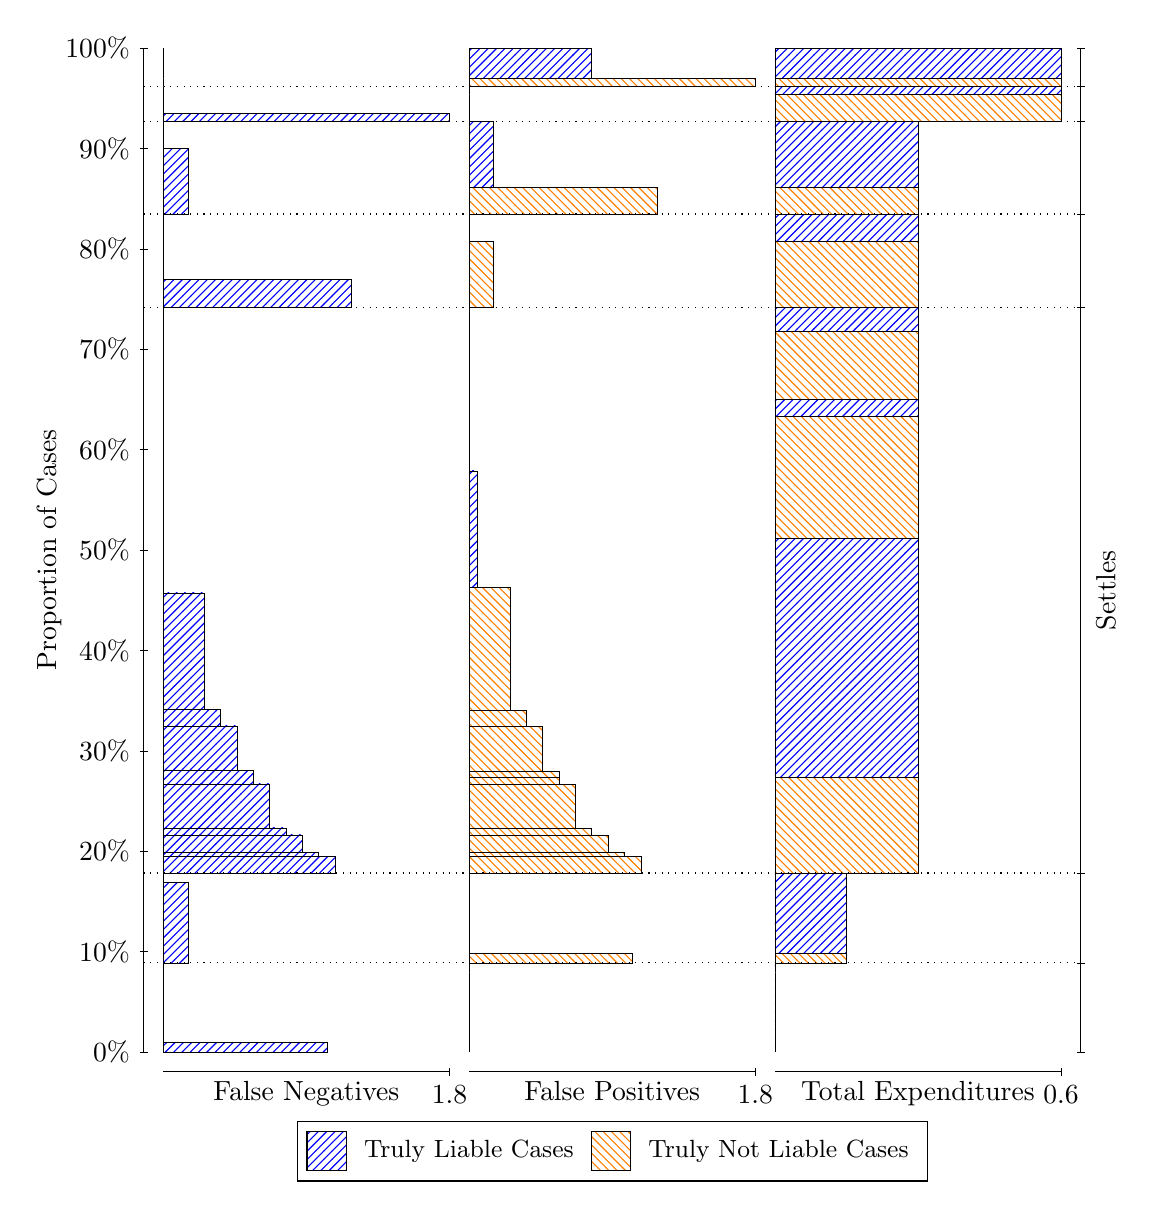
\begin{tikzpicture}
\draw[black, very thin] (1.5,1.75) -- (1.5,14.5);
\node[rotate=90, anchor=center] at (0.3, 8.125) {Proportion of Cases};
\draw[black, very thin] (1.45,1.75) -- (1.55,1.75);
\node[anchor=east] at (1.45, 1.75) {0\%};
\draw[black, very thin] (1.45,3.025) -- (1.55,3.025);
\node[anchor=east] at (1.45, 3.025) {10\%};
\draw[black, very thin] (1.45,4.3) -- (1.55,4.3);
\node[anchor=east] at (1.45, 4.3) {20\%};
\draw[black, very thin] (1.45,5.575) -- (1.55,5.575);
\node[anchor=east] at (1.45, 5.575) {30\%};
\draw[black, very thin] (1.45,6.85) -- (1.55,6.85);
\node[anchor=east] at (1.45, 6.85) {40\%};
\draw[black, very thin] (1.45,8.125) -- (1.55,8.125);
\node[anchor=east] at (1.45, 8.125) {50\%};
\draw[black, very thin] (1.45,9.4) -- (1.55,9.4);
\node[anchor=east] at (1.45, 9.4) {60\%};
\draw[black, very thin] (1.45,10.675) -- (1.55,10.675);
\node[anchor=east] at (1.45, 10.675) {70\%};
\draw[black, very thin] (1.45,11.95) -- (1.55,11.95);
\node[anchor=east] at (1.45, 11.95) {80\%};
\draw[black, very thin] (1.45,13.225) -- (1.55,13.225);
\node[anchor=east] at (1.45, 13.225) {90\%};
\draw[black, very thin] (1.45,14.5) -- (1.55,14.5);
\node[anchor=east] at (1.45, 14.5) {100\%};

\draw[black, very thin] (13.4,1.75) -- (13.4,14.5);
\draw[black, very thin] (13.35,1.75) -- (13.45,1.75);
\node[anchor=west] at (13.35, 1.75) {};
\draw[black, very thin] (13.35,2.881) -- (13.45,2.881);
\node[anchor=west] at (13.35, 2.881) {};
\draw[black, very thin] (13.35,4.0227) -- (13.45,4.0227);
\node[anchor=west] at (13.35, 4.0227) {};
\draw[black, very thin] (13.35,11.205) -- (13.45,11.205);
\node[anchor=west] at (13.35, 11.205) {};
\draw[black, very thin] (13.35,12.392) -- (13.45,12.392);
\node[anchor=west] at (13.35, 12.392) {};
\draw[black, very thin] (13.35,13.569) -- (13.45,13.569);
\node[anchor=west] at (13.35, 13.569) {};
\draw[black, very thin] (13.35,14.01) -- (13.45,14.01);
\node[anchor=west] at (13.35, 14.01) {};
\draw[black, very thin] (13.35,14.5) -- (13.45,14.5);
\node[anchor=west] at (13.35, 14.5) {};

\draw[black, very thin, pattern color=blue, pattern=north east lines] (1.75,1.75) rectangle (3.8262,1.869);
\draw[black, very thin, pattern color=orange, pattern=north west lines] (1.75,1.869) rectangle (1.75,2.881);
\draw[black, very thin, pattern color=blue, pattern=north east lines] (1.75,2.881) rectangle (2.0614,3.9042);
\draw[black, very thin, pattern color=orange, pattern=north west lines] (1.75,3.9042) rectangle (1.75,4.0227);
\draw[black, very thin, pattern color=blue, pattern=north east lines] (1.75,4.0227) rectangle (3.93,4.2379);
\draw[black, very thin, pattern color=blue, pattern=north east lines] (1.75,4.2379) rectangle (3.7224,4.2882);
\draw[black, very thin, pattern color=blue, pattern=north east lines] (1.75,4.2882) rectangle (3.5148,4.5056);
\draw[black, very thin, pattern color=blue, pattern=north east lines] (1.75,4.5056) rectangle (3.3071,4.5969);
\draw[black, very thin, pattern color=blue, pattern=north east lines] (1.75,4.5969) rectangle (3.0995,5.1556);
\draw[black, very thin, pattern color=blue, pattern=north east lines] (1.75,5.1556) rectangle (2.8919,5.3236);
\draw[black, very thin, pattern color=blue, pattern=north east lines] (1.75,5.3236) rectangle (2.6843,5.891);
\draw[black, very thin, pattern color=blue, pattern=north east lines] (1.75,5.891) rectangle (2.4767,6.0979);
\draw[black, very thin, pattern color=blue, pattern=north east lines] (1.75,6.0979) rectangle (2.269,7.5799);
\draw[black, very thin, pattern color=orange, pattern=north west lines] (1.75,7.5799) rectangle (1.75,11.205);
\draw[black, very thin, pattern color=blue, pattern=north east lines] (1.75,11.205) rectangle (4.1376,11.557);
\draw[black, very thin, pattern color=orange, pattern=north west lines] (1.75,11.557) rectangle (1.75,12.392);
\draw[black, very thin, pattern color=blue, pattern=north east lines] (1.75,12.392) rectangle (2.0614,13.226);
\draw[black, very thin, pattern color=orange, pattern=north west lines] (1.75,13.226) rectangle (1.75,13.569);
\draw[black, very thin, pattern color=blue, pattern=north east lines] (1.75,13.569) rectangle (5.3833,13.67);
\draw[black, very thin, pattern color=orange, pattern=north west lines] (1.75,13.67) rectangle (1.75,14.01);
\draw[black, very thin, pattern color=orange, pattern=north west lines] (1.75,14.01) rectangle (1.75,14.111);
\draw[black, very thin, pattern color=blue, pattern=north east lines] (1.75,14.111) rectangle (1.75,14.5);
\draw[black, very thin, pattern color=orange, pattern=north west lines] (5.6333,1.75) rectangle (5.6333,2.762);
\draw[black, very thin, pattern color=blue, pattern=north east lines] (5.6333,2.762) rectangle (5.6333,2.881);
\draw[black, very thin, pattern color=orange, pattern=north west lines] (5.6333,2.881) rectangle (7.7095,2.9996);
\draw[black, very thin, pattern color=blue, pattern=north east lines] (5.6333,2.9996) rectangle (5.6333,4.0227);
\draw[black, very thin, pattern color=orange, pattern=north west lines] (5.6333,4.0227) rectangle (7.8133,4.2321);
\draw[black, very thin, pattern color=orange, pattern=north west lines] (5.6333,4.2321) rectangle (7.6057,4.2805);
\draw[black, very thin, pattern color=orange, pattern=north west lines] (5.6333,4.2805) rectangle (7.3981,4.4983);
\draw[black, very thin, pattern color=orange, pattern=north west lines] (5.6333,4.4983) rectangle (7.1905,4.589);
\draw[black, very thin, pattern color=orange, pattern=north west lines] (5.6333,4.589) rectangle (6.9829,5.1466);
\draw[black, very thin, pattern color=orange, pattern=north west lines] (5.6333,5.1466) rectangle (6.7752,5.2329);
\draw[black, very thin, pattern color=orange, pattern=north west lines] (5.6333,5.2329) rectangle (6.7752,5.3105);
\draw[black, very thin, pattern color=orange, pattern=north west lines] (5.6333,5.3105) rectangle (6.5676,5.8806);
\draw[black, very thin, pattern color=orange, pattern=north west lines] (5.6333,5.8806) rectangle (6.36,6.0926);
\draw[black, very thin, pattern color=orange, pattern=north west lines] (5.6333,6.0926) rectangle (6.1524,7.6474);
\draw[black, very thin, pattern color=blue, pattern=north east lines] (5.6333,7.6474) rectangle (5.7371,9.1295);
\draw[black, very thin, pattern color=blue, pattern=north east lines] (5.6333,9.1295) rectangle (5.6333,11.205);
\draw[black, very thin, pattern color=orange, pattern=north west lines] (5.6333,11.205) rectangle (5.9448,12.04);
\draw[black, very thin, pattern color=blue, pattern=north east lines] (5.6333,12.04) rectangle (5.6333,12.392);
\draw[black, very thin, pattern color=orange, pattern=north west lines] (5.6333,12.392) rectangle (8.021,12.735);
\draw[black, very thin, pattern color=blue, pattern=north east lines] (5.6333,12.735) rectangle (5.9448,13.569);
\draw[black, very thin, pattern color=orange, pattern=north west lines] (5.6333,13.569) rectangle (5.6333,13.909);
\draw[black, very thin, pattern color=blue, pattern=north east lines] (5.6333,13.909) rectangle (5.6333,14.01);
\draw[black, very thin, pattern color=orange, pattern=north west lines] (5.6333,14.01) rectangle (9.2667,14.111);
\draw[black, very thin, pattern color=blue, pattern=north east lines] (5.6333,14.111) rectangle (7.1905,14.5);
\draw[black, very thin, pattern color=orange, pattern=north west lines] (9.5167,1.75) rectangle (9.5167,2.762);
\draw[black, very thin, pattern color=blue, pattern=north east lines] (9.5167,2.762) rectangle (9.5167,2.881);
\draw[black, very thin, pattern color=orange, pattern=north west lines] (9.5167,2.881) rectangle (10.425,2.9996);
\draw[black, very thin, pattern color=blue, pattern=north east lines] (9.5167,2.9996) rectangle (10.425,4.0227);
\draw[black, very thin, pattern color=orange, pattern=north west lines] (9.5167,4.0227) rectangle (11.333,5.2329);
\draw[black, very thin, pattern color=blue, pattern=north east lines] (9.5167,5.2329) rectangle (11.333,8.2681);
\draw[black, very thin, pattern color=orange, pattern=north west lines] (9.5167,8.2681) rectangle (11.333,9.823);
\draw[black, very thin, pattern color=blue, pattern=north east lines] (9.5167,9.823) rectangle (11.333,10.038);
\draw[black, very thin, pattern color=orange, pattern=north west lines] (9.5167,10.038) rectangle (11.333,10.898);
\draw[black, very thin, pattern color=blue, pattern=north east lines] (9.5167,10.898) rectangle (11.333,11.205);
\draw[black, very thin, pattern color=orange, pattern=north west lines] (9.5167,11.205) rectangle (11.333,12.04);
\draw[black, very thin, pattern color=blue, pattern=north east lines] (9.5167,12.04) rectangle (11.333,12.392);
\draw[black, very thin, pattern color=orange, pattern=north west lines] (9.5167,12.392) rectangle (11.333,12.735);
\draw[black, very thin, pattern color=blue, pattern=north east lines] (9.5167,12.735) rectangle (11.333,13.569);
\draw[black, very thin, pattern color=orange, pattern=north west lines] (9.5167,13.569) rectangle (13.15,13.909);
\draw[black, very thin, pattern color=blue, pattern=north east lines] (9.5167,13.909) rectangle (13.15,14.01);
\draw[black, very thin, pattern color=orange, pattern=north west lines] (9.5167,14.01) rectangle (13.15,14.111);
\draw[black, very thin, pattern color=blue, pattern=north east lines] (9.5167,14.111) rectangle (13.15,14.5);
\draw[black, dotted] (1.5,2.881) -- (13.4,2.881);
\draw[black, dotted] (1.5,4.0227) -- (13.4,4.0227);
\draw[black, dotted] (1.5,11.205) -- (13.4,11.205);
\draw[black, dotted] (1.5,12.392) -- (13.4,12.392);
\draw[black, dotted] (1.5,13.569) -- (13.4,13.569);
\draw[black, dotted] (1.5,14.01) -- (13.4,14.01);
\draw[black, very thin] (1.75,1.5) -- (5.3833,1.5);
\node[anchor=north] at (3.5667, 1.5) {False Negatives};
\draw[black, very thin] (5.3833,1.45) -- (5.3833,1.55);
\node[anchor=north] at (5.3833, 1.45) {1.8};

\draw[black, very thin] (5.6333,1.5) -- (9.2667,1.5);
\node[anchor=north] at (7.45, 1.5) {False Positives};
\draw[black, very thin] (9.2667,1.45) -- (9.2667,1.55);
\node[anchor=north] at (9.2667, 1.45) {1.8};

\draw[black, very thin] (9.5167,1.5) -- (13.15,1.5);
\node[anchor=north] at (11.333, 1.5) {Total Expenditures};
\draw[black, very thin] (13.15,1.45) -- (13.15,1.55);
\node[anchor=north] at (13.15, 1.45) {0.6};



\node[black, centered, rotate=90] at (13.72, 7.6137) {Settles};





\draw (7.449999999999999,1.5) node[draw=none] (baseCoordinate) {};
\begin{scope}[align=center]
        \matrix[scale=0.5, draw=black, below=0.5cm of baseCoordinate, nodes={draw}, column sep=0.1cm]{
            \node[rectangle, draw, minimum width=0.5cm, minimum height=0.5cm, pattern=north east lines, pattern color=blue] {}; &
            \node[draw=none, font=\small] (B) {Truly Liable Cases}; &
            \node[rectangle, draw, minimum width=0.5cm, minimum height=0.5cm, pattern=north west lines, pattern color=orange] {}; &
            \node[draw=none, font=\small] (B) {Truly Not Liable Cases}; \\
            };
\end{scope}

\end{tikzpicture}
\end{document}